%\documentclass[review]{cvpr}
\documentclass[final]{cvpr}

%\usepackage{cvpr}
\usepackage{times}
\usepackage{epsfig}
\usepackage{graphicx}
\usepackage{amsmath}
\usepackage{amssymb}
\usepackage{subfigure}
\usepackage{overpic}

\usepackage{enumitem}
\setenumerate[1]{itemsep=0pt,partopsep=0pt,parsep=\parskip,topsep=5pt}
\setitemize[1]{itemsep=0pt,partopsep=0pt,parsep=\parskip,topsep=5pt}
\setdescription{itemsep=0pt,partopsep=0pt,parsep=\parskip,topsep=5pt}

% Include other packages here, before hyperref.

% If you comment hyperref and then uncomment it, you should delete
% egpaper.aux before re-running latex.  (Or just hit 'q' on the first latex
% run, let it finish, and you should be clear).
\usepackage[pagebackref=true,breaklinks=true,colorlinks,bookmarks=false]{hyperref}


%\cvprfinalcopy % *** Uncomment this line for the final submission

\def\cvprPaperID{159} % *** Enter the CVPR Paper ID here
\def\confYear{CVPR 2020}


\newcommand{\cmm}[1]{\textcolor[rgb]{0,0.6,0}{CMM: #1}}
\newcommand{\todo}[1]{{\textcolor{red}{\bf [#1]}}}
\newcommand{\alert}[1]{\textcolor[rgb]{.6,0,0}{#1}}

\newcommand{\IT}{IT\cite{98pami/Itti}}
\newcommand{\MZ}{MZ\cite{03ACMMM/Ma_Contrast-based}}
\newcommand{\GB}{GB\cite{conf/nips/HarelKP06}}
\newcommand{\SR}{SR\cite{07cvpr/hou_SpectralResidual}}
\newcommand{\FT}{FT\cite{09cvpr/Achanta_FTSaliency}}
\newcommand{\CA}{CA\cite{10cvpr/goferman_context}}
\newcommand{\LC}{LC\cite{06acmmm/ZhaiS_spatiotemporal}}
\newcommand{\AC}{AC\cite{08cvs/achanta_salient}}

\newcommand{\HC}{HC-maps }
\newcommand{\RC}{RC-maps }
\newcommand{\Lab}{$L^*a^*b^*$}

\newcommand{\vnudge}{\vspace*{-.1in}}
%\newcommand{\vnudge}{\vspace*{-2pt}}

\newcommand{\mypara}[1]{\paragraph{#1.}}

%\renewcommand{\baselinestretch}{0.995}


\graphicspath{{figures/}}

% Pages are numbered in submission mode, and unnumbered in camera-ready
%\ifcvprfinal\pagestyle{empty}\fi
\setcounter{page}{409}

\begin{document}

%%%%%%%%% TITLE

\title{Global Contrast based Salient Region Detection}

\author{Ming-Ming Cheng$^{1}$\quad Guo-Xin Zhang$^{1}$ \quad Niloy J. Mitra$^{2}$
    \quad Xiaolei Huang$^{3}$  \quad Shi-Min Hu$^{1}$  \\
    $^{1}$ TNList, Tsinghua University \quad \quad
    $^2$ KAUST   \quad \quad $^3$ Lehigh University\\
    %{\tt \small [chengmingvictor, zgx.net, niloym]@gmail.com \quad xih206@lehigh.edu \quad shimin@tsinghua.edu.cn}
    {\tt \small chengmingvictor@gmail.com}
}

\maketitle
% \thispagestyle{empty}

%%%%%%%%% ABSTRACT
\begin{abstract}
%
Reliable estimation of visual saliency allows appropriate processing of images without prior
knowledge of their contents, and thus remains an important step in many computer vision tasks
including image segmentation, object recognition, and adaptive compression.
%
We propose a regional contrast based saliency extraction algorithm,
which simultaneously evaluates global contrast differences and spatial coherence.
%
The proposed algorithm is simple, efficient, and yields full resolution saliency maps.
%
Our algorithm consistently outperformed existing saliency detection methods, yielding
higher precision and better recall rates, when evaluated using one of the largest
publicly available data sets.
%
We also demonstrate how the extracted saliency map can be used to create high quality
segmentation masks for subsequent image processing.


\end{abstract}




%%%%%%%%% BODY TEXT %%%%%%%%%%%%%%%%%%%%%%%%%%%%%%%%%%%%%%%%
\section{Introduction}\label{sec:Introduction}

Humans routinely and effortlessly judge the importance of image regions, and focus
attention on important parts.
%
Computationally detecting such salient image regions remains a significant goal,
as it allows preferential allocation of computational resources in subsequent image analysis and synthesis.
%
Extracted saliency maps are widely used in many computer vision applications including object-of-interest
image segmentation~\cite{06TCSVT/han_unsupervised,06josa/KoN_InterestSegmentation},
object recognition~\cite{04cvpr/RutishauserWWKP},  adaptive compression of images~\cite{00CE/christopoulos_jpeg},
content-aware image editing~\cite{TOG/Wang08,09cgf/ZhangC,wu-2010-resizing,10vc/Ding}, and image retrieval~\cite{tog09/ChenCT_Sketch2Photo}.


\begin{figure}[t!]
   \begin{overpic}[width=\columnwidth]{teaser.pdf}
    \end{overpic}
    \caption{Given input images~(top), a global contrast analysis is used
    to compute high resolution saliency maps~(middle), which can be used to
    produce masks~(bottom) around regions of interest.
    }\label{fig:teaser} \vnudge
\end{figure}


\begin{figure*}[t!]
   \begin{overpic}[width=\textwidth]{all_comparisons.pdf} \small
   \put(0.3,0){(a)~original}
   \put(10,0){(b)~\IT}
   \put(18.3,0){(c)~\MZ}
   \put(27.5,0){(d)~\GB}
   \put(37,0){(e)~\SR}
   \put(46.5,0){(f)~\AC}
   \put(55.5,0){(g)~\CA}
   \put(65,0){(h)~\FT}
   \put(73.5,0){(i)~\LC}
   \put(84,0){(j)~HC}
   \put(93,0){(k)~RC}
   \end{overpic}
   \caption{Saliency maps computed by different state-of-the-art methods~(b-i),
     and with our proposed HC~(j) and RC methods~(k). Most results
     highlight edges, or are of low resolution.
     See also Figure~\ref{fig:VisualComparison} (and our project webpage).
   }\label{fig:cmp1vAll} \vnudge
\end{figure*}


Saliency originates from visual uniqueness, unpredictability, rarity, or surprise, and is often
attributed to variations in image attributes like color, gradient, edges, and boundaries.
%
Visual saliency, being closely related to how we perceive and process visual stimuli, is
investigated by multiple disciplines including cognitive
psychology~\cite{55ARP/Teuber_physiological,04nature/Wolfe_attributesVisual},
neurobiology~\cite{95ARN/DesimoneNeuralMachanisms,09biology/eyeMovement}, and computer
vision~\cite{98pami/Itti,09cvpr/Achanta_FTSaliency}.
%
Theories of human attention hypothesize that the human vision system only processes parts of an image in detail,
while leaving others nearly unprocessed.
%
Early work by Treisman and Gelade~\cite{80cogSc/Treisman_featureIntegration}, Koch and
Ullman~\cite{85HN/KochVisualAttention}, and subsequent attention theories proposed by Itti, Wolfe
and others, suggest two stages of visual attention: fast, pre-attentive, bottom-up, data driven
saliency extraction; and slower, task dependent, top-down, goal driven saliency extraction.




We focus on bottom-up data driven saliency detection using image contrast.
%
It is widely believed that human cortical cells may be \emph{hard wired} to preferentially respond
to high contrast stimulus in their receptive fields~\cite{03neuron/Reynolds_attentionSaliency}.
%
We propose contrast analysis for extracting high-resolution, full-field saliency maps based on the
following observations:
\begin{itemize}
  \item A global contrast based method, which separates a large-scale object from its surroundings,
    is preferred over local contrast based methods producing high saliency values at or near object edges.
  \item Global considerations enable assignment of comparable saliency values to similar image regions,
    and can uniformly highlight entire objects.
  \item Saliency of a region depends mainly on its contrast to the nearby regions,
    while contrasts to distant regions are less significant.
  \item Saliency maps should be fast and easy to generate to allow processing of
    large image collections, and facilitate efficient image classification and retrieval.
\end{itemize}


We propose a \emph{histogram-based contrast method}~(HC) to measure saliency.
%
\HC assign pixel-wise saliency values based simply on color separation from all other image
pixels to produce full resolution saliency maps. We use a histogram-based approach for efficient processing,
while employing a smoothing procedure to control quantization artifacts.
%
Note that our algorithm is targeted towards natural scenes,
and maybe suboptimal for extracting saliency of highly textured scenes (see \figref{fig:challenging_maps}).


As an improvement over HC-maps, we incorporate spatial relations to produce
\emph{region-based contrast}~(RC) maps where we first segment the input image into
regions, and then assign saliency values to them. The saliency value of a region is
now calculated using a global contrast score, measured by the region's
contrast and spatial distances to other regions in the image.


We have extensively evaluated our methods on publicly available benchmark data sets, and compared
our methods with (eight) state-of-the-art saliency methods
~\cite{98pami/Itti,03ACMMM/Ma_Contrast-based,06acmmm/ZhaiS_spatiotemporal,conf/nips/HarelKP06,07cvpr/hou_SpectralResidual,08cvs/achanta_salient,09cvpr/Achanta_FTSaliency,10cvpr/goferman_context}
as well as with manually produced ground truth annotations\footnote{Results for 1000 images and
prototype software are available at the project webpage:
\href{http://cg.cs.tsinghua.edu.cn/people/~cmm/saliency/}{http://cg.cs.tsinghua.edu.cn/people/\%7Ecmm/saliency/}}.
%
The experiments show significant improvements over previous methods both in precision and recall rates.
%
Overall, compared with HC-maps, \RC produce better precision and recall rates, but at the cost
of increased computations. Encouragingly, we observe that the saliency cuts extracted
using our saliency maps are, in most cases, comparable to manual annotations.
%
We also present application of the extracted saliency maps to segmentation,
context aware resizing, and non-photo realistic rendering.




%%%%%%%%%%%%%%%%%%%%%%%%%%%%%%%%%%%%%%%%%%%%%%%%%%%%%%%%%%%%%%%%%%%%%%%%%%%%%%%%%
\section{Related Work}
\label{sec:RelatedWorks}

We focus on relevant literature targeting pre-attentive bottom-up saliency detection,
which may be biologically motivated, or purely computational, or involve both aspects.
%
Such methods utilize low-level processing to determine the contrast of image regions to their surroundings,
using feature attributes such as intensity, color, and edges~\cite{09cvpr/Achanta_FTSaliency}.
%
We broadly classify the algorithms into local and global schemes.


Local contrast based methods investigate the rarity of image regions with respect to (small) local neighborhoods.
%
Based on the highly influential biologically inspired \emph{early representation} model introduced
by Koch and Ullman~\cite{85HN/KochVisualAttention}, Itti et al.~\cite{98pami/Itti} define image
saliency using central-surrounded differences across multi-scale image features.
%
Ma and Zhang~\cite{03ACMMM/Ma_Contrast-based} propose an alternative local contrast
analysis for generating saliency maps, which is then extended using a fuzzy growth model.
%
Harel et al.~\cite{conf/nips/HarelKP06} normalize the feature maps of Itti et al., to highlight
conspicuous parts and permit combination with other importance maps.
%
Liu et al.~\cite{10pami/Liu_Learning} find multi-scale contrast by linearly combining contrast
in a Gaussian image pyramid.
%
More recently, Goferman et al.~\cite{10cvpr/goferman_context} simultaneously model local
low-level clues, global considerations, visual organization rules, and high-level
features to highlight salient objects along with their contexts.
%
Such methods using local contrast tend to produce higher saliency values near edges instead of uniformly
highlighting salient objects (see \figref{fig:cmp1vAll}).


Global contrast based methods evaluate saliency of an image region using its contrast
with respect to the entire image.
%
Zhai and Shah~\cite{06acmmm/ZhaiS_spatiotemporal} define pixel-level saliency based on a pixel's contrast to all other pixels.
However, for efficiency they use only luminance information, thus ignoring distinctiveness clues in other channels.
%
Achanta et al.~\cite{09cvpr/Achanta_FTSaliency} propose a frequency tuned method that
directly defines pixel saliency using a pixel's color difference from the average image
color. The elegant approach, however, only considers first order average color, which
can be insufficient to analyze complex variations common in natural images.
%
In Figures~\ref{fig:VisualComparison} and~\ref{fig:plots}, we show qualitative and
quantitative weaknesses of such approaches. Furthermore, these methods ignore spatial
relationships across image parts, which can be critical for reliable and coherent
saliency detection (see \secref{sec:Experiment}).


%%%%%%%%%%%%%%%%%%%%%%%%%%%%%%%%%%%%%%%%%%%%%%%%%%%%%%%%%%
\section{Histogram Based Contrast}\label{sec:HC}


Based on the observation from biological vision that the vision system is sensitive to contrast in visual signal,
we propose a histogram-based contrast~(HC) method to define saliency values
for image pixels using color statistics of the input image.
%
Specifically, the saliency of a pixel is defined using its color contrast to all other pixels in the image,
i.e., the saliency value of a pixel $I_k$ in image $I$ is defined as,
\begin{equation}\label{equ:PixelColorContrast}
    S(I_k) = \sum_{\forall I_i \in I} D(I_k, I_i),
\end{equation}
where $D(I_k, I_i)$ is the color distance metric between pixels $I_k$ and $I_i$ in the
\Lab space (see also~\cite{06acmmm/ZhaiS_spatiotemporal}).
%
%
\equref{equ:PixelColorContrast} can be expanded by pixel order to have the following
form,
\begin{equation}\label{equ:PixelCCPixelOrder}
    S(I_k) = D(I_k, I_1) + D(I_k, I_2) + \cdots + D(I_k, I_N),
\end{equation}where $N$ is the number of pixels in image $I$.
%
It is easy to see that pixels with the same color value have the same saliency value
under this definition, since the measure is oblivious to spatial relations. Hence,
rearranging \equref{equ:PixelCCPixelOrder} such that the terms with the same color value
$c_j$ are grouped together, we get saliency value for each color as,
\begin{equation}\label{equ:PixelCCColorOrder}
    S(I_k) = S(c_l) = \sum_{j=1}^{n}{f_j D(c_l, c_j)},
\end{equation}
where $c_l$ is the color value of pixel $I_k$, $n$ is the number of distinct pixel colors, and
$f_j$ is the probability of pixel color $c_j$ in image $I$.
%
Note that in order to prevent salient region color statistics from being corrupted by
similar colors from other regions, one can develop a similar scheme using varying window
masks. However, given the strict efficiency requirement, we take the simple global
approach.


\begin{figure}
  	\begin{overpic}[width=\columnwidth]{histogram.pdf}
    \end{overpic}
    \caption{Given an input image~(left), we compute its color histogram~(middle).
      Corresponding histogram bin colors are shown in the lower bar.
      The quantized image~(right) uses only  $43$ histogram bin colors
      and still retains sufficient visual quality for saliency detection.
    }\label{fig:colorFre} \vnudge
\end{figure}


%%%%%%%%%%%%%%%%%%%%%%%%%%%%%%%%%%%%%%%%%%%%%%%
\vnudge
\mypara{Histogram based speed up} Naively evaluating the saliency value for each image
pixel using \equref{equ:PixelColorContrast} takes $O(N^2)$ time, which is
computationally too expensive even for medium sized images.
%
The equivalent representation in \equref{equ:PixelCCColorOrder}, however, takes $O(N) + O(n^2)$ time,
implying that computational efficiency can be improved to $O(N)$ if $O(n^2) \leq O(N)$.
%
Thus, the key to speed up is to reduce the number of pixel colors in the image.
However, the true-color space contains $256^3$ possible colors,
which is typically larger than the number of image pixels.


Zhai and Shah~\cite{06acmmm/ZhaiS_spatiotemporal} reduce the number of colors, $n$,
by only using luminance. In this way, $n^2=256^2$ (typically $256^2 \ll N$).
However, their method has the disadvantage that the distinctiveness of color information is ignored.
%
In this work, we use the full color space instead of luminance only.
To reduce the number of colors needed to consider, we first quantize each color channel to have 12 different values,
which reduces the number of colors to $12^3=1728$.
%
Considering that color in a natural image typically covers only a small portion of the full color space,
we further reduce the number of colors by ignoring less frequently occurring colors.
%
By choosing more frequently occurring colors and ensuring these colors cover the colors of more
than $95\%$ of the image pixels, we typically are left with around $n=85$ colors (see
\secref{sec:Experiment} for experimental details).
%
The colors of the remaining pixels, which comprise fewer than $5\%$ of the image pixels,
are replaced by the closest colors in the histogram. A typical example of such
quantization is shown in \figref{fig:colorFre}.
%
Note that again due to efficiency requirements we select the simple histogram based quantization
instead of optimizing for an image specific color palette.


\begin{figure}
    \centering
    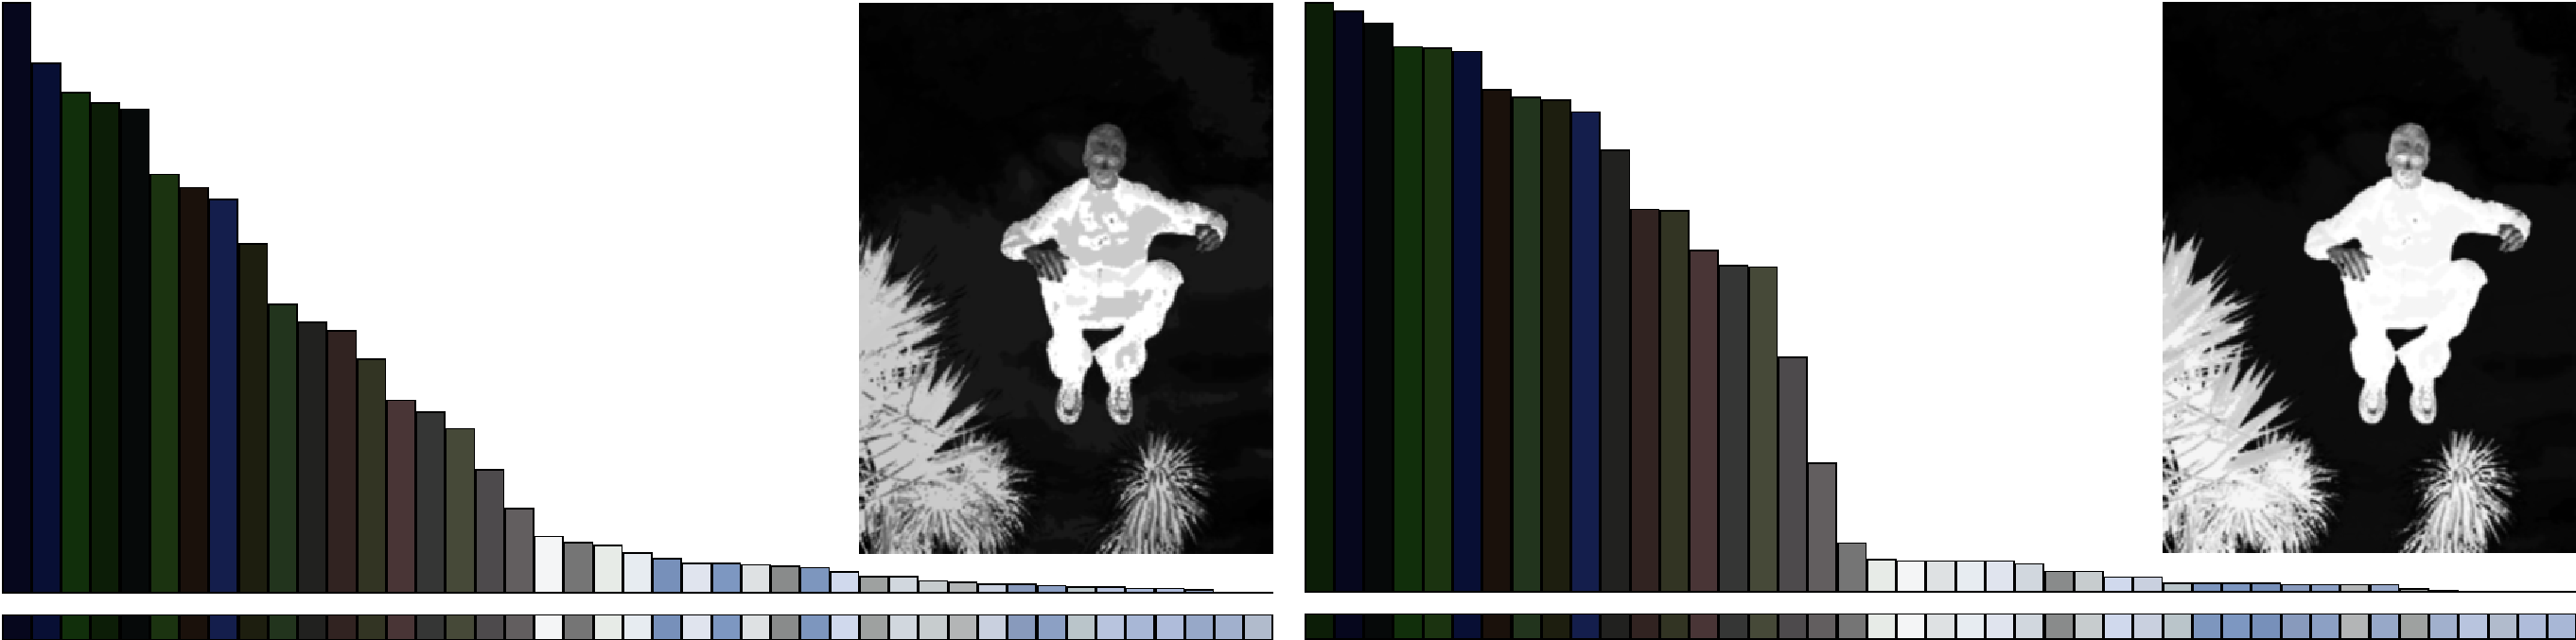
\includegraphics[width=\columnwidth]{histogram_saliency.pdf}
    \caption{Saliency of each color, normalized to the range $[0,1]$,
        before~(left) and after~(right) color space smoothing.
        Corresponding saliency maps are shown in the respective insets.
    }\label{fig:HCSmoothing} \vnudge
\end{figure}


%%%%%%%%%%%%%%%%%%%%%%%%%%%%%%%%%%%%%%%%%%%%%%
\vnudge
\mypara{Color space smoothing}
Although we can efficiently compute color contrast by building a compact color histogram
using color quantization and choosing more frequent colors,
the quantization itself may introduce artifacts.
%
Some similar colors may be quantized to different values.
In order to reduce noisy saliency results caused by such randomness,
we use a smoothing procedure to refine the saliency value for each color.
%
We replace the saliency value of each color by the weighted average of the saliency
values of similar colors (measured by \Lab distance).
%
This is actually a smoothing process in the color feature space. Typically we choose
$m=n/4$ nearest colors to refine the saliency value of color $c$ by,
\begin{equation}\label{equ:smoothing}
    S'(c) = \frac{1}{(m-1)T} \sum_{i=1}^{m} (T-D(c, c_i))S(c_i)
\end{equation}
where $T=\sum_{i=1}^{m} D(c, c_i)$ is the sum of distances between color $c$ and its
$m$ nearest neighbors $c_i$, and the normalization factor comes from
%\begin{equation*}\label{equ:smoothingN}
    $\sum_{i=1}^{m} (T-D(c, c_i))=(m-1)T.$
%\end{equation*}
%
Note that we use a linearly-varying smoothing weight $(T-D(c, c_i))$ to assign
larger weights to colors closer to $c$ in the color feature space.
%
In our experiments, we found that such linearly-varying weights are better than Gaussian
weights, which fall off too sharply.
%
\figref{fig:HCSmoothing} shows the typical effect of color space smoothing with the
corresponding histograms sorted by decreasing saliency values.
%
Note that similar histogram bins are closer to each other after such  smoothing,
indicating that similar colors have higher likelihood of being assigned similar saliency values,
thus reducing quantization artifacts (see \figref{fig:plots}).


\vnudge
\mypara{Implementation details}
To quantize the color space into $12^3$ different colors, we uniformly divide each color
channel into 12 different levels.
%
While the quantization of colors is performed in the RGB color space, we measure color
differences in the \Lab color space because of its perceptual accuracy.
%
However, we do not perform quantization directly in the \Lab color space since not all colors in
the range $L^*\in[0, 100]$, and $a^*, b^*\in[-127,127]$ necessarily correspond to real colors.
%
Experimentally we observed worse quantization artifacts using direct \Lab color space
quantization.
%
Best results were obtained by quantization in the RGB space while measuring distance in the \Lab
color space, as opposed to performing both quantization and distance calculation in a
single color space, either RGB or \Lab.



%%%%%%%%%%%%%%%%%%%%%%%%%%%%%%%%%%%%%%%%%%%%%%%%%%%%%%%%%%
\section{Region Based Contrast}

\begin{figure}
    \centering
    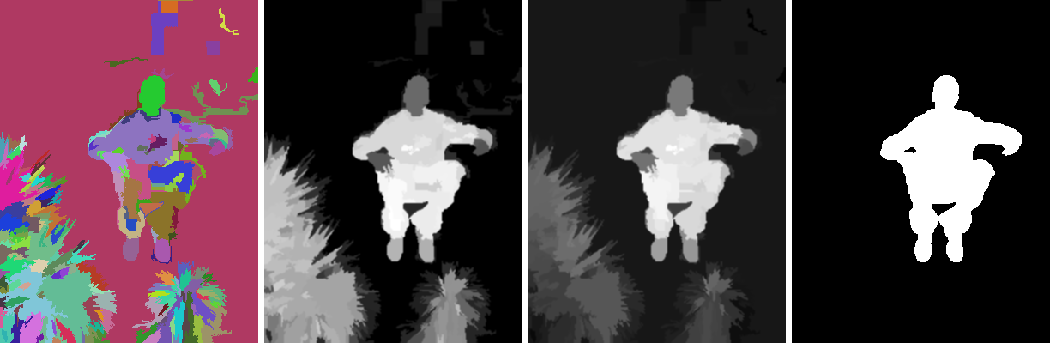
\includegraphics[width=\columnwidth]{region_contrast.pdf}\\
    \caption{Image regions generated by Felzenszwalb and Huttenlocher's
      segmentation method~\cite{04ijcv/felzenszwalb_efficient}~(left),
      region contrast based segmentation with~(left-middle) and without~(right-middle) distance weighting.
      Incorporating the spatial context, we get a high quality saliency cut~(right) comparable to
      human labeled ground truth.
    }\label{fig:regContrast} \vnudge
\end{figure}


Humans pay more attention to those image regions that contrast strongly with their
surroundings~\cite{03neuroscience/luminanceContrast}.
%
Besides contrast, spatial relationships play an  important role in human attention.
%
High contrast to its surrounding regions is usually stronger evidence for
saliency of a region than high contrast to far-away regions.
%
Since directly introducing spatial relationships when computing pixel-level contrast is
computationally expensive, we introduce a   contrast analysis method, \emph{region contrast} (RC),
so as to integrate spatial relationships into region-level contrast computation.
%
In RC, we first segment the input image into regions, then compute color contrast at the region level,
and define the saliency for each region as the weighted sum of the region's contrasts
to all other regions in the image.
%
The weights are set according to the spatial distances with farther regions being assigned smaller
weights.


%%%%%%%%%%%%%%%%%%%%%%%%%%%%%%%%%%%%%%%%%%%%%%%%%%%%%%%%%%

\vnudge
\mypara{Region contrast by sparse histogram comparison}
We first segment the input image into regions using a graph-based image segmentation
method \cite{04ijcv/felzenszwalb_efficient}.
%
Then we build the color histogram for each region as in \secref{sec:HC}.
%
For a region $r_k$, we compute its saliency value by measuring its color contrast to all other
regions in the image,
\begin{equation}\label{equ:regContrastSaliency}
    S(r_k) = \sum_{r_k \neq r_i} w(r_i)  D_r(r_k, r_i),
\end{equation}
where $w(r_i)$ is the weight of region $r_i$ and $D_r(\cdot, \cdot)$ is the color distance metric
between the two regions.
%
Here we use the number of pixels in $r_i$ as $w(r_i)$ to emphasize color contrast to bigger regions.
%
The color distance between two regions $r_1$ and $r_2$ is defined as,
\begin{equation}\label{equ:regContrast}
    D_r(r_1, r_2) = \sum_{i=1}^{n_1} \sum_{j=1}^{n_2} f(c_{1,i}) f(c_{2,j}) D(c_{1,i}, c_{2,j})
\end{equation}
where $f(c_{k,i})$ is the probability of the $i$-th color $c_{k,i}$ among all $n_k$ colors in the
$k$-th
 region $r_k$, $k=\{1,2\}$.
%
%Similarly we define $c_{2,j}$, $n_2$ and $f(c_{2,j})$ for region $r_2$.
%
Note that we use the probability of a color in the probability density function (i.e. normalized color histogram) of the region as the weight for this color to emphasize more the color differences between dominant colors.


Storing and calculating the regular matrix format histogram for each region is inefficient since
each region typically contains a small number of colors in the color histogram of the whole image.
%
Instead, we use a sparse histogram representation for efficient storage and computation.


%%%%%%%%%%%%%%%%%%%%%%%%%%%%%%%%%%%%%%%%%%%%%%%%%%%%%%%%%%
\vnudge
\mypara{Spatially weighted region contrast} We further incorporate spatial information by
introducing a spatial weighting term in \equref{equ:regContrastSaliency}   to increase the effects
of closer regions and decrease the effects of farther regions.
%
Specifically, for any region $r_k$, the spatially weighted region contrast based saliency is
defined as:
\begin{equation}\label{equ:regContrastSpatial}
    S(r_k) =  \sum_{r_k \neq r_i} \exp({-D_s(r_k, r_i)/\sigma_s^2})  w(r_i)  D_r(r_k, r_i)
\end{equation}
where $D_s(r_k, r_i)$ is the spatial distance between regions $r_k$ and $r_i$, and $\sigma_s$
controls the strength of spatial weighting.
%
Larger values of $\sigma_s$ reduce the effect of spatial weighting
so that contrast to farther regions would contribute more to the saliency of the current region.
%
The spatial distance between two regions is defined as the Euclidean distance between their
centroids. In our implementation, we use $\sigma_s^2 = 0.4$ with pixel
coordinates normalized to $[0, 1]$.



%%%%%%%%%%%%%%%%%%%%%%%%%%%%%%%%%%%%%%%%%%%%%%%%%%%%%%%%%%%%%%%%%%%%%%
\section{Experimental Comparisons}\label{sec:Experiment}

\begin{figure*}[t!]
   \begin{overpic}[width=\textwidth]{comparison.pdf} \small
   \put(3,0){(a)~original}
   \put(18.5,0){(b)~LC}
   \put(33,0){(c)~CA}
   \put(48,0){(d)~FT}
   \put(60,0){(e)~\HC}
   \put(74,0){(f)~\RC}
   \put(90,0){(g)~RCC}
   \end{overpic}
   \caption{Visual comparison of saliency maps. (a)~original images, saliency maps produced using
       (b)~Zhai and Shah~\cite{06acmmm/ZhaiS_spatiotemporal},
       (c)~Goferman et al.~\cite{10cvpr/goferman_context},
       (d) Achanta et al.~\cite{09cvpr/Achanta_FTSaliency},
       (e) our HC and (f)~RC methods, and (g)~RC-based saliency cut results.
       Our methods generate uniformly highlighted salient regions. (See our project webpage for all results on the full benchmark dataset.)
   }\label{fig:VisualComparison} \vnudge
\end{figure*}

We have evaluated the results of our approach on the publicly available database provided
by Achanta et al. \cite{09cvpr/Achanta_FTSaliency}.
%
To the best of our knowledge, the database is the largest of its kind, and has ground truth in the
form of accurate human-marked labels for salient regions.
%
We compared the proposed global contrast based methods  with $8$ state-of-the-art saliency detection methods.
%
Following~\cite{09cvpr/Achanta_FTSaliency}, we selected these methods according to:
number of citations (\IT ~and \SR), recency (\GB, SR, \AC, \FT ~and \CA), variety (IT is
biologically-motivated, \MZ~is purely computational, GB is hybrid, SR works in the frequency
domain, AC and FT output full resolution saliency maps), and being related to
our approach (\LC).


We used our methods and the others to compute saliency maps for all the 1000 images in
the database.
%
\tabref{tab:TimeEfficency} compares the average time taken by each method.
%
Our algorithms,  HC and RC, are implemented in C++.
%
For the other methods namely IT, GB, SR, FT and CA, we used the authors' implementations,
while for LC, we implemented the algorithm in C++ since we could not find the authors'
implementation.
%
For typical natural images, our HC method needs $O(N)$ computation time and is sufficiently
efficient for real-time applications. In contrast, our RC variant is slower as it requires image
segmentation~\cite{04ijcv/felzenszwalb_efficient}, but produces superior quality saliency maps.

\begin{table*}
    \centering
    \begin{tabular}{l|c|c|c|c|c|c|c|c|c|c} \hline\hline
      Method  &  \IT   &  \MZ  &   \GB  &  \SR   &  \FT  &  \AC  &  \CA   & \LC   &  HC   &  RC   \\ \hline
      Time(s) & 0.611  & 0.070 & 1.614  & 0.064  & 0.016 & 0.109 &  53.1  & 0.018 & 0.019 & 0.253 \\ \hline
      Code    & Matlab & C++   & Matlab & Matlab &  C++  &  C++  & Matlab &  C++  &  C++  &  C++  \\ \hline\hline
    \end{tabular}
    \caption{Average time taken to compute a saliency map for images in the database
        by Achanta et al.~\cite{09cvpr/Achanta_FTSaliency}. Most images in the
        database~(see our project webpage) have resolution $400\times300$.
        Algorithms were tested using a Dual Core 2.6 GHz machine with 2GB RAM.
    } \label{tab:TimeEfficency}
\end{table*}


\begin{figure*}
  \centering
  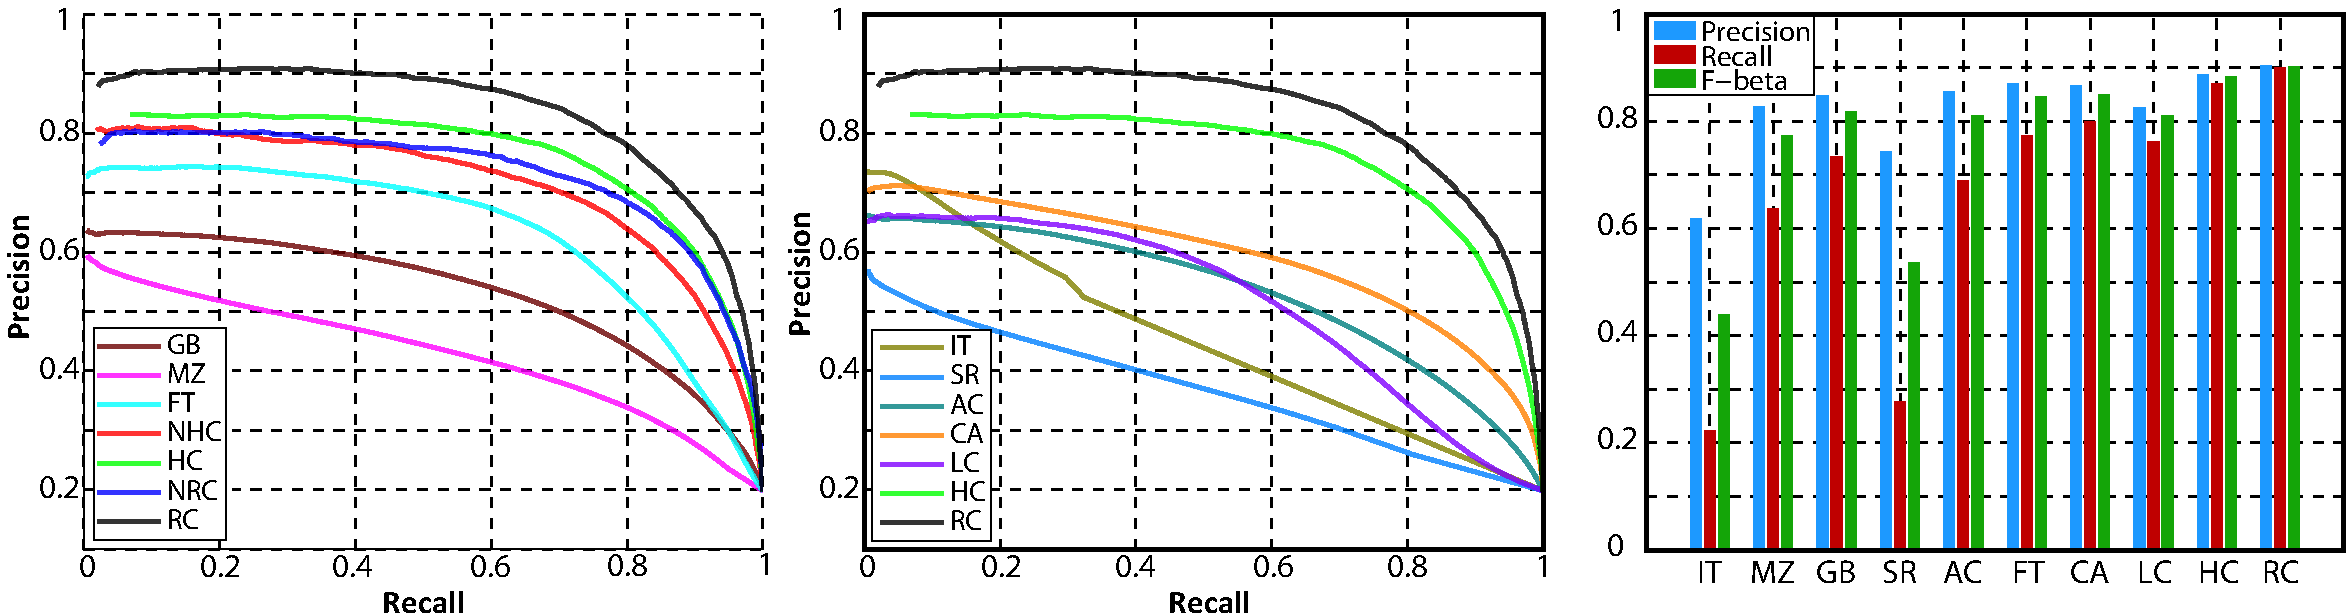
\includegraphics[width=\textwidth]{plots.pdf}
  \caption{Precision-recall curves for naive thresholding of saliency maps
    using 1000 publicly available benchmark images. (Left, middle)~Different options
    of our method compared with \GB, \MZ,  \FT, \IT, \SR, \AC, \CA, and \LC.
    NHC denotes a naive version of our HC method with color space smoothing disabled, and
    NRC denotes our RC method with spatial related weighting disabled.
    %
    (Right)~Precision-recall bars for our saliency cut algorithm using
    different saliency maps as initialization. Our method RC shows high
    precision, recall, and $F_{\beta}$ values over the 1000-image database. (Please refer to
    our project webpage for the respective result images.)
  } \label{fig:plots} \vnudge
\end{figure*}

In order to comprehensively evaluate the accuracy of our methods for salient object
segmentation, we performed two experiments using different objective comparison measures.
%
In the first experiment, to segment salient objects and calculate precision and recall
curves~\cite{07cvpr/hou_SpectralResidual}, we binarized the saliency map using every possible fixed
threshold, similar to the fixed thresholding experiment in~\cite{09cvpr/Achanta_FTSaliency}.
%
In the second experiment, we segment salient objects by iteratively applying
GrabCut~\cite{04tog/rother_grabcut} initialized using thresholded saliency maps, as we will describe later.
%
We also use the obtained saliency maps as importance weighting for content aware image
resizing and non-photo realistic rendering.



%%%%%%%%%%%%%%%%%%%%%%%%%%%%%%%%%%%%%%%%%%%%%%%%%%%%%%%%%
\vnudge
\mypara{Segmentation by fixed thresholding}
The simplest way to get a binary segmentation of salient objects is to
threshold the saliency map with a threshold $T_f \in [0, 255]$.
%
To reliably compare how well various saliency detection methods highlight salient regions in images,
we vary the threshold $T_f$ from $0$ to $255$. \figref{fig:plots} shows the resulting precision vs. recall curves.
%
We also present the  benefits of adding the color space smoothing and spatial weighting
schemes, along with objective comparison with other saliency extraction methods.
%
Visual comparison of saliency maps obtained by the various methods can be seen in
Figures~\ref{fig:cmp1vAll} and \ref{fig:VisualComparison}. %(All test results on the whole database are included as
%supplementary material.)


The precision and recall curves clearly show that our methods outperform the other eight methods.
%
The extremities of the precision vs. recall curve are interesting: At maximum recall
where $T_f = 0$, all pixels are retained as positives, i.e., considered to be
foreground, so all the methods have the same precision and recall values; precision
$0.2$ and recall $1.0$ at this point indicate that, on average, there are $20\%$ image
pixels belonging to the ground truth salient regions.
%
At the other end, the minimum recall values of our methods are higher than those of the other
methods, because the saliency maps computed by our methods are smoother and contain more
pixels with the saliency value $255$.



%%%%%%%%%%%%%%%%%%%%%%%%%%%%%%%%%%%%%%%%%%%%%
\vnudge
\mypara{Saliency cut}
We now consider the use of the computed saliency map to assist in salient object segmentation.
%
Saliency maps have been previously employed for unsupervised object segmentation:
%
Ma and Zhang~\cite{03ACMMM/Ma_Contrast-based} find rectangular salient regions
by fuzzy region growing on their saliency maps.
%
Ko and Nam~\cite{06josa/KoN_InterestSegmentation} select salient regions using a support
vector machine trained on image segment features, and then cluster these
regions to extract salient objects.
%
Han et al.~\cite{06TCSVT/han_unsupervised} model color, texture, and edge features in a Markov
random field framework to grow salient object regions from seed values in the saliency maps.
%
More recently, Achanta et al.~\cite{09cvpr/Achanta_FTSaliency} average saliency values within
image segments produced by mean-shift segmentation, and then find salient objects by identifying
image segments that have average saliency above a threshold that is set to be twice the mean
saliency value of the entire image.


\begin{figure}[b!]
    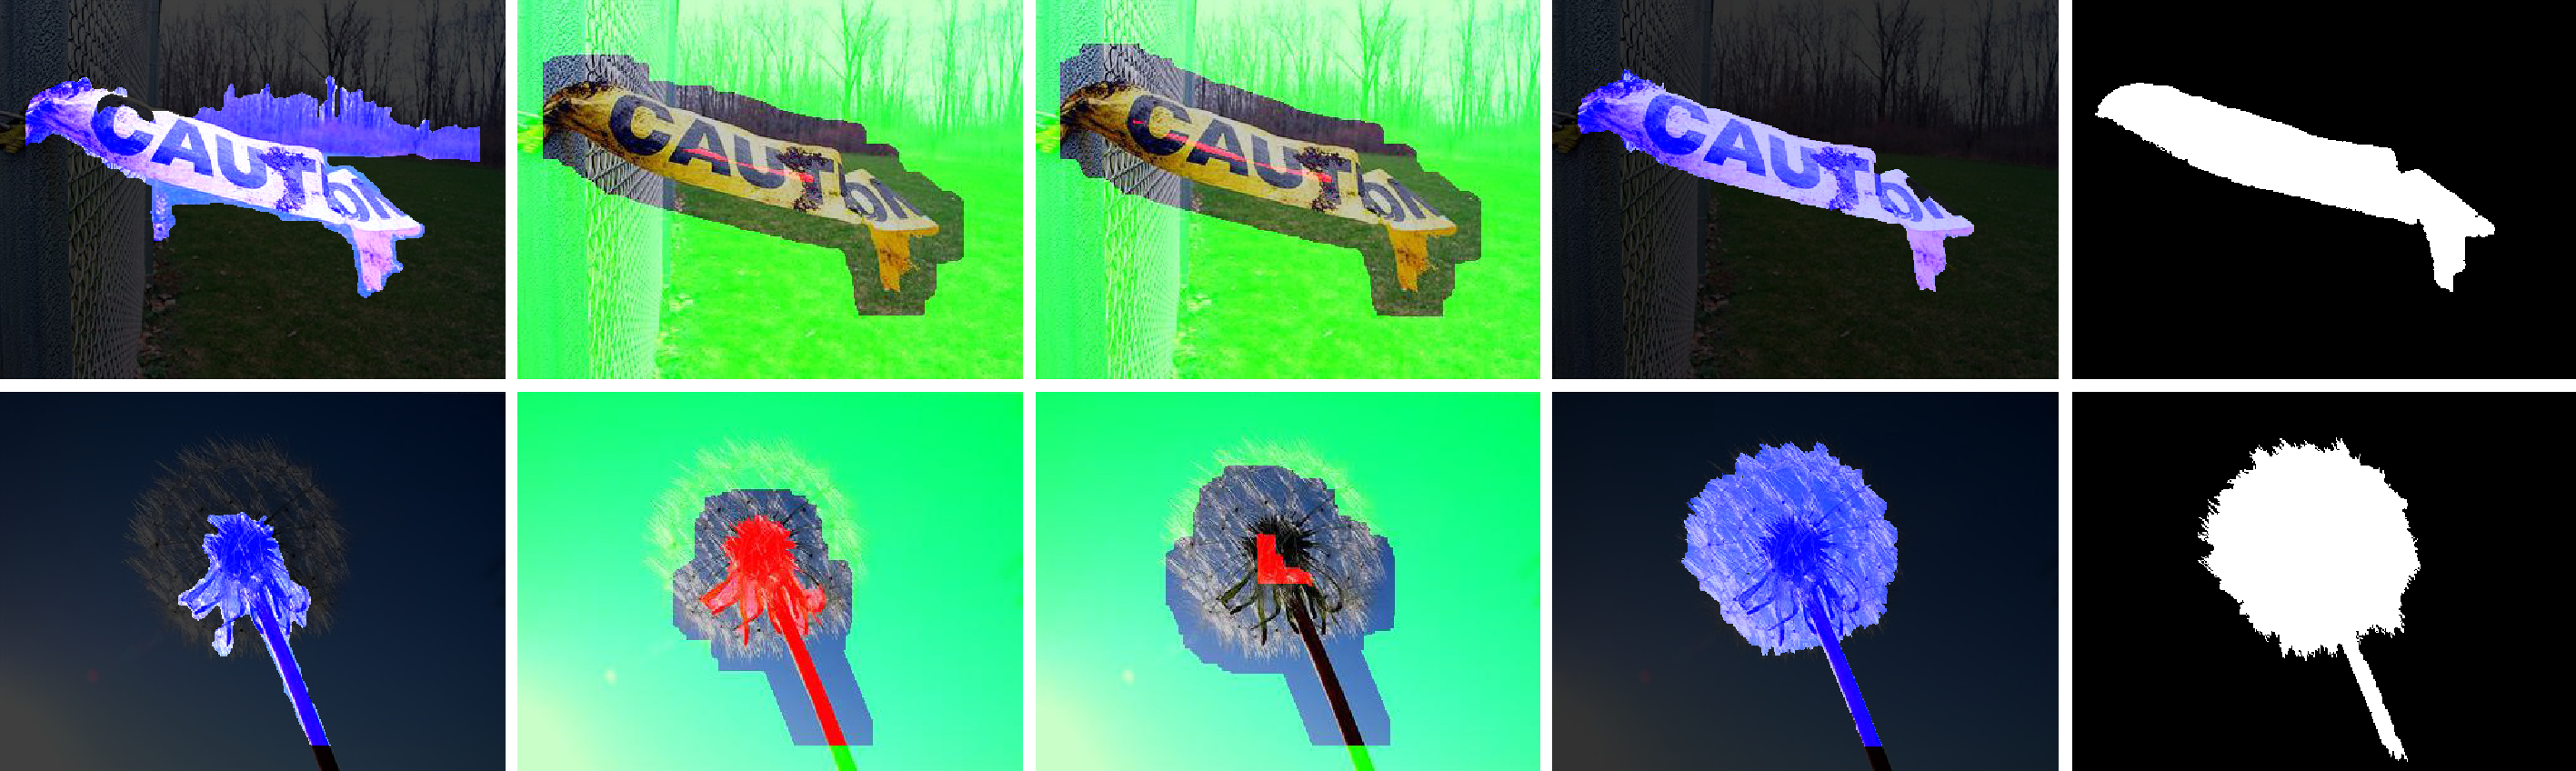
\includegraphics[width=\columnwidth]{saliency_cut.pdf}
    \caption{Saliency Cut. (Left to right) Initial segmentation, trimap after first iteration,
        trimap after second iteration, final segmentation, and manually labeled ground truth.
        In the segmented images, blue is foreground, gray is background, while in
         the trimaps, foreground is red, background is green, and unknown regions are left unchanged.
    }\label{fig:AttCutSteps} \vnudge
\end{figure}

\begin{figure*}
  \begin{overpic}[width=\linewidth]{cut_compare.pdf}\small
    \put(3,0){(a)~original}
    \put(17,0){(b)~\LC}
    \put(32,0){(c)~\CA}
    \put(46,0){(d)~\FT}
    \put(60,0){(e)~\HC}
    \put(74,0){(f)~\RC}
    \put(87,0){(g)~ground truth}
  \end{overpic}
  \caption{Saliency cut using different saliency maps for initialization.
    The respective saliency maps are shown in \figref{fig:VisualComparison}.
  }\label{fig:cutCmp} \vnudge
\end{figure*}


In our approach, we iteratively apply GrabCut \cite{04tog/rother_grabcut} to refine the
segmentation result initially obtained by thresholding the saliency map (see
\figref{fig:AttCutSteps}).
%
Instead of manually selecting a rectangular region to initialize the process, as in classical GrabCut,
we automatically initialize GrabCut using a segmentation obtained by binarizing the saliency map using a fixed threshold; the threshold is chosen empirically to be the threshold that gives $95\%$ recall rate in our fixed thresholding experiments.


Once initialized, we iteratively run GrabCut to improve the saliency cut result. (At most $4$ iterations are run in our experiments.)
%
After each iteration, we use dilation and erosion operations on the current segmentation
result to get a new trimap for the next GrabCut iteration.
%
As shown in \figref{fig:AttCutSteps}, the region outside the dilated region is set to
background, the region inside the eroded region is set to foreground, and the remaining
areas are set to unknown in the trimap.
%
GrabCut, which by itself is an iterative process using Gaussian mixture models and graph cut,
helps to refine salient object regions at each step.
%
Regions closer to an initial salient object region are more likely to be part of that salient object than far-away regions.
%
Thus, our new initialization enables GrabCut to include nearby salient regions,
and exclude non-salient regions according to color feature dissimilarity.
%
In the implementation, we set a narrow image-border region (15 pixels wide) to be always in the background in order to
avoid slow convergence in the border region.


\figref{fig:AttCutSteps} shows two examples of our saliency cut algorithm.
%
In the flag example, unwanted regions are correctly excluded during GrabCut iterations.
%
In the flower example, our saliency cut method successfully expanded the initial salient regions
(obtained directly from the saliency map) and converged to an accurate segmentation result.

To objectively evaluate our new saliency cut method using our RC-map as initialization,
we compare our results with results obtained by coupling iterative GrabCut with initializations
from saliency maps computed by other methods.
%
For consistency, we binarize each such saliency map using a threshold that gives $95\%$
recall rate in the corresponding fixed thresholding experiment (see \figref{fig:plots}). A visual comparison of the results is shown in \figref{fig:cutCmp}.
%
Average precision, recall, and $F$-Measure are compared over the entire ground-truth
database~\cite{09cvpr/Achanta_FTSaliency}, with the $F$-Measure defined as:
\begin{equation}\label{equ:FMeasure}
    F_{\beta} = \frac{(1+\beta^2)Precision \times Recall}{\beta^2 \times Precision + Recall}.
\end{equation}
We use $\beta^2 = 0.3$ as in Achanta et al.~\cite{09cvpr/Achanta_FTSaliency} to weigh
precision more than recall.
%
As can be seen from the comparison (see Figures~\ref{fig:plots}-right and \ref{fig:cutCmp}),
saliency cut using our RC and HC saliency maps significantly outperform other methods.
%
Compared with the state-of-the-art results on this database by Achanta et al. (precision = $75\%$, recall = $83\%$), we achieved better accuracy (precision = $90\%$, recall = $90\%$). (Our demo software is available at our project webpage.)


%%%%%%%%%%%%%%%%%%%%%%%%%%%%%%%%%%%%%%%%%%%%%%%%%%%%
\begin{figure}[t!]
   \begin{overpic}[width=\columnwidth]{contentAware_application.pdf} \small
   \put(3,0){original}
   \put(21,0){CA}
   \put(31,0){RC}
   \put(48,0){original}
   \put(75,0){CA}
   \put(90,0){RC}
    \end{overpic}
    \caption{Comparison of content aware image resizing~\cite{09cgf/ZhangC} results
        using \CA  saliency maps and our RC saliency maps.
    }\label{fig:Resizing} \vnudge
\end{figure}




\vnudge
\mypara{Content aware image resizing} In image re-targeting, saliency maps are usually used to
specify relative importance across image parts (see also~\cite{09_image_resize}).
%
We experimented with using our saliency maps in the image resizing method proposed by Zhang et al.~\cite{09cgf/ZhangC}\footnote{The authors' original implementation is publicly available.}, which
distributes distortion energy to relatively non-salient regions of an image while
preserving both global and local image features.
%
Figure~\ref{fig:Resizing} compares the resizing results using our \RC with the results using \CA ~saliency maps.
Our RC saliency maps help produce better resizing results since the saliency values in salient object regions are piece-wise smooth,
which is important for energy based resizing methods.
%
CA saliency maps, having higher saliency values at object boundaries, are less suitable for
applications like resizing, which require entire salient objects to be uniformly highlighted.




%%%%%%%%%%%%%%%%%%%%%%%%%%%%%%%%%%%%%%%%%%%%%%%%%
\vnudge
\mypara{Non-photorealistic rendering}
%
Artists often abstract images and highlight meaningful parts of an image while masking out
unimportant regions~\cite{99/zeki_innerVision}.
%
Inspired by this observation, a number of non-photorealistic rendering~(NPR) efforts use saliency
maps to generate interesting  effects~\cite{02tog/decarlo_stylization}.
%
We experimentally compared our work with the most related, state-of-the-art saliency detection
algorithm~\cite{09cvpr/Achanta_FTSaliency} in the context of a recent NPR
technique~\cite{10pg/Huang_Zhang} (see \figref{fig:NPR}).
%
Our \RC give better saliency masks, which help the NPR method to better preserve details
in important image parts and region boundaries, while smoothing out others.



%%%%%%%%%%%%%%%%%%%%%%%%%%%%%%%%%%%%%%%%%%%%%%%%%%%%
\begin{figure}[t!]
   \begin{overpic}[width=\columnwidth]{npr_application2.pdf} \small
     \end{overpic}
    \caption{(Middle, right)~\FT$ $ and RC saliency maps are used respectively
        for stylized rendering~\cite{10pg/Huang_Zhang} of an input image~(left).
        Our method produces a better saliency map, see insets, resulting in
        improved preservation of details, e.g., around the head and the fence regions.
    }\label{fig:NPR} \vnudge
\end{figure}


\begin{figure}[t!]
   \begin{overpic}[width=\columnwidth]{challenging_maps.pdf} \small
     \end{overpic}
    \caption{ Challenging examples for our histogram based methods involve non-salient regions with
    similar colors as the salient parts~(top), or an image with textured background~(bottom).
    (Left to right)~Input image, HC-map, HC saliency cut, RC-map, RC saliency cut.
    } \label{fig:challenging_maps} \vnudge
\end{figure}



%%%%%%%%%%%%%%%%%%%%%%%%%%%%%%%%%%%%%%%%%%%%%%%%%
\vnudge
\section{Conclusions and Future Work}\label{sec:Conclusion}

We presented global contrast based saliency computation methods, namely  Histogram based
Contrast~(HC) and spatial information-enhanced Region based Contrast~(RC).
%
While the HC method is fast and generates results with fine details, the RC method generates
spatially coherent high quality saliency maps at the cost of reduced computational efficiency.
%
We evaluated our methods on the largest publicly available data set and compared our scheme with
eight other state-of-the-art methods.
%
Experiments indicate the proposed schemes to be superior in terms of both precision and recall,
while still being simple and efficient.


In the future, we plan to investigate  efficient algorithms that incorporate spatial relationships
in saliency computation while preserving fine details in the resulting saliency maps. Also, it is
desirable to develop saliency detection algorithms to handle cluttered and textured background,
which could introduce artifacts to our global histogram based approach.
%(although we did not encounter such images in the database).
%
Finally, it may be beneficial to incorporate high level factors like human faces, symmetry into saliency maps.
We believe the proposed saliency maps can be used for efficient object detection \cite{06TCSVT/han_unsupervised},
reliable image classification, robust image scene analysis~\cite{journal/tog/ChengZMHH10},
leading to improved image retrieval \cite{tog09/ChenCT_Sketch2Photo}.

%\paragraph{Acknowledgements.} This research was supported by the
%National Basic Research Project of China (NO. 2011CB302205),
%the Natural Science Foundation of China (NO. U0735001)
%and the National High Technology Research and Development Program of China (NO. 2009AA01Z327).

\vnudge
\paragraph{Acknowledgements.} This research was supported by the
973 Program (2011CB302205), the 863 Program (2009AA01Z327), the Key Project of
S\&T (2011ZX01042-001-002), and NSFC (U0735001).
Ming-Ming Cheng was funded by Google PhD fellowship, IBM PhD fellowship,
and New PhD Researcher Award (Ministry of Edu., CN).

{\small
\bibliographystyle{ieee}
\bibliography{Saliency}
}

\end{document}
